%{{{fold} fix for acrobat reader
\pdfobjcompresslevel=1
%{endfold}}}


\documentclass[a4paper]{article}

%{{{fold} packages
\usepackage[margin=20mm]{geometry}

\usepackage[utf8]{inputenc}
\usepackage[T1]{fontenc}
\usepackage{libertine}

\usepackage[french]{babel}

\usepackage{tikz}
\usetikzlibrary{calc, shadows, backgrounds}
\usepackage{graphicx}

\usepackage{tabularx}
\usepackage{enumerate}
\usepackage{hyperref}
\usepackage{needspace}

\usepackage{ifthen}

\usepackage{amsmath}
\usepackage{mathabx}
%{endfold}}}

%{{{fold} disable some warnings
\pdfsuppresswarningpagegroup=1
%{endfold}}}

\title{Projet : Roborally}
\author{}
\date{}

%{{{fold} ignore warnings
\pdfsuppresswarningpagegroup=1
%{endfold}}}

%{{{fold} basic commands
\newcommand{\li}{\linewidth}

\addto\extrasfrench{
  \let\subsectionautorefname\sectionautorefname
  \let\subsubsectionautorefname\sectionautorefname
}
%{endfold}}}

%{{{fold} drawing
\newlength{\tilewidth}
\setlength{\tilewidth}{7mm}

\newcommand{\tile}[3][0]{%
  \foreach \elem in {#3}
  {
    \draw[x=\tilewidth, y=\tilewidth] 
    (#2) node[rotate=#1] {\includegraphics[width=\tilewidth]{Images/\elem.pdf}} ;
  } ;
}

\newcommand{\textile}[1]{%
  \begin{tikzpicture}[baseline, anchor=base]
    \tile{0,0}{#1}
  \end{tikzpicture}
}

\tikzset{
  inline board/.style=
  {
    x=\tilewidth, y=\tilewidth,
    baseline={($( current bounding box.center) - (0,0.3em) $)}
  },
  board node/.style=
  {
    draw, thick, rounded corners, fill=white, drop shadow, 
    inner sep = 2pt, outer sep = 0pt
  },
  arrow label/.style=
  {
    draw, thick, rounded corners, fill=white
  }
}

\newcommand{\keystroke}[1]{%
  \tikz[baseline=(key.base)]
    \node[%
      draw,
      fill=white,
      drop shadow={shadow xshift=0.25ex,shadow yshift=-0.25ex,fill=black,opacity=0.5},
      rectangle,
      rounded corners=2pt,
      inner sep=1pt,
      minimum width=5mm,
      minimum height=5mm
    ](key) {\textbf{#1}\strut}
  ;
}

\newcommand{\mouseclick}[1]{%
  \tikz[baseline=(symbol.base)]
  \node[inner sep = 0pt, outer sep = 0pt] (symbol)%
  {%
    $\vcenter{\hbox{%
        \ifthenelse{#1 = 1}%
        {%
          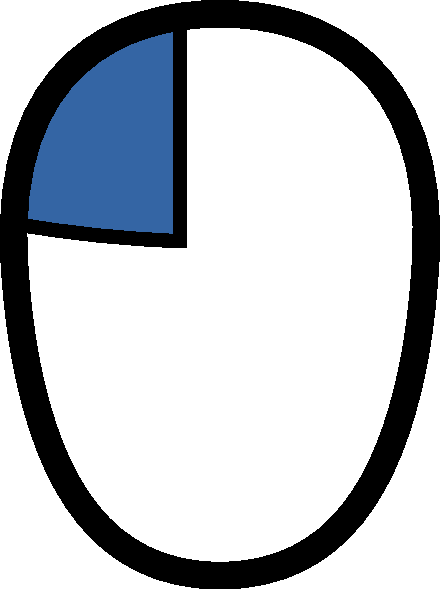
\includegraphics[width=4mm]{Images/mouse_left_button.pdf}%
        }%
        {%
          \ifthenelse{#1 = 2}%
          {%
            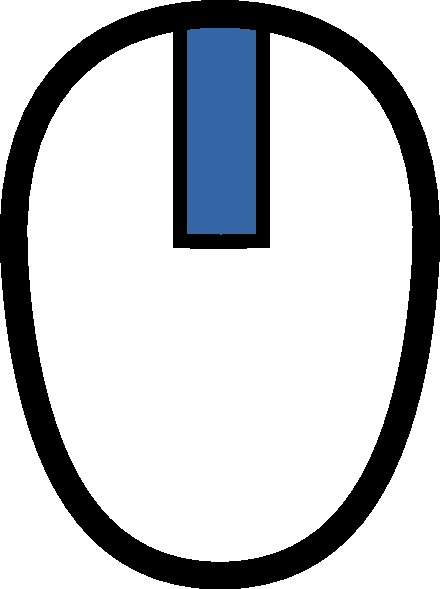
\includegraphics[width=4mm]{Images/mouse_middle_button.pdf}%
          }%
          {%
            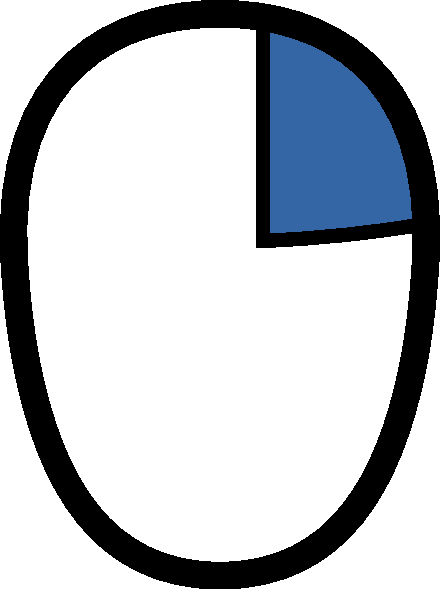
\includegraphics[width=4mm]{Images/mouse_right_button.pdf}%
          }%
        }%
    }}$%
  } ;%
}
%{endfold}}}

\begin{document}

\noindent
\begin{minipage}{0.5\li}
  Université Claude Bernard, Lyon 1

  Algorithmique, programmation et complexité -- LIFAP6
\end{minipage}
\hfill
\begin{minipage}{0.4\li}
  \raggedright
  License Sciences et Technologies, L3

  2020 -- 2021, semestre de printemps
\end{minipage}

{\let\newpage\relax\maketitle}

\section{Introduction}

\paragraph{}Roborally est un jeu de société élaboré par Richard Garfield en
1994. Le but de ce projet est de créer un programme capable de jouer de manière
autonome à une version simplifiée du jeu. Chaque joueur incarne un petit robot
qui doit trouver son chemin dans une usine. L'usine est parsemée de tapis
roulants et de plateaux tournants qui vont perturber les déplacements du robot.
Roborally est une course, et le but est donc de se déplacer le plus rapidement
possible. Ce projet a pour but de vous faire appliquer les notions sur les
graphes et les algorithmes de plus court chemin associés pour calculer
automatiquement les meilleures séquences de coups possibles pour déplacer le
robot.

En terminant la première partie de ce projet, vous devriez normalement être
capable de formuler un problème de plus court chemin à l'aide de la théorie des
graphes, et d'appliquer l'algorithme de Dijkstra pour obtenir une solution à ce
problème. Il est important que l'algorithme utilisé soit bien l'algorithme de
Dijkstra et non une variante de votre cru.

En abordant la seconde partie, vous pourrez faire preuve de créativité pour
définir la stratégie du robot dans des situations de jeu plus complexes. Vous
serez amenés à vous questionner sur les performances de votre solution, en terme
de complexité spatiale et temporelle et en terme de qualité du résultat obtenu.

\section{Règles du jeu}

\subsection{Robot}
\label{sec:robotactions}

\paragraph{} Votre robot est défini par une position et une orientation. Pour
déplacer le robot, sept actions sont possibles : avancer de une, deux ou trois
cases, reculer de une case, tourner à gauche ou a droite, faire demi-tour. La
direction dans laquelle le robot avance ou recule est déterminée par son
orientation. Tourner le robot permet de changer son orientation. Les effets des
différentes actions sont illustrés ci-dessous.

\begin{center}
  \begin{tabular}{l|ll}
    \textbf{Action} & \textbf{Avant} & \textbf{Après} \\
    \hline
    Avancer d'une case &
    \begin{tikzpicture}[inline board]
      \tile{0,0}{background,robot}
      \tile{1,0}{background}
    \end{tikzpicture} &
    \begin{tikzpicture}[inline board]
      \tile{0,0}{background}
      \tile{1,0}{background,robot}
    \end{tikzpicture} \\
    Avancer de deux cases &
    \begin{tikzpicture}[inline board]
      \tile{0,0}{background,robot}
      \tile{1,0}{background}
      \tile{2,0}{background}
    \end{tikzpicture} &
    \begin{tikzpicture}[inline board]
      \tile{0,0}{background}
      \tile{1,0}{background}
      \tile{2,0}{background,robot}
    \end{tikzpicture} \\
    Avancer de trois cases &
    \begin{tikzpicture}[inline board]
      \tile{0,0}{background,robot}
      \tile{1,0}{background}
      \tile{2,0}{background}
      \tile{3,0}{background}
    \end{tikzpicture} &
    \begin{tikzpicture}[inline board]
      \tile{0,0}{background}
      \tile{1,0}{background}
      \tile{2,0}{background}
      \tile{3,0}{background,robot}
    \end{tikzpicture} \\
    Reculer d'une case &
    \begin{tikzpicture}[inline board]
      \tile{0,0}{background}
      \tile{1,0}{background,robot}
    \end{tikzpicture} &
    \begin{tikzpicture}[inline board]
      \tile{0,0}{background,robot}
      \tile{1,0}{background}
    \end{tikzpicture} \\
    Tourner à gauche &
    \begin{tikzpicture}[inline board]
      \tile{0,0}{background,robot}
    \end{tikzpicture} &
    \begin{tikzpicture}[inline board]
      \tile{0,0}{background}
      \tile[90]{0,0}{robot}
    \end{tikzpicture} \\
    Tourner à droite &
    \begin{tikzpicture}[inline board]
      \tile{0,0}{background,robot}
    \end{tikzpicture} &
    \begin{tikzpicture}[inline board]
      \tile{0,0}{background}
      \tile[-90]{0,0}{robot}
    \end{tikzpicture} \\
    Faire demi tour &
    \begin{tikzpicture}[inline board]
      \tile{0,0}{background,robot}
    \end{tikzpicture} &
    \begin{tikzpicture}[inline board]
      \tile{0,0}{background}
      \tile[180]{0,0}{robot}
    \end{tikzpicture} \\
    \hline
  \end{tabular}
\end{center}

Lorsque le robot sort du plateau de jeu, il est détruit et ne peut plus faire la
moindre action.

\subsection{Plateau de jeu}

\paragraph{}Après chaque déplacement du robot, les éléments du plateau sont mis
en œuvre. Ces éléments peuvent être des tapis roulants, des tapis roulants
rapides ou des plateaux tournants. Il ne vous est normalement pas nécessaire de
comprendre dans le détail comment ces éléments fonctionnent, car le code fourni
comprend un programme qui traite ces éléments pour vous. Dans tous les exemples
fournis, le robot est placé dans une situation initiale, puis il est illustré
dans son état après avoir effectué l'action « avancer d'une case » puis avoir
appliqué les éléments du plateau.

\paragraph{}Dans l'ordre, les tapis roulants sont appliqués, puis les plateaux
tournants.  Les plateaux tournants font tourner votre robot, vers la droite ou
vers la gauche selon leur type.

\vspace{5mm}
\begin{minipage}[t]{0.45\li}
  \centering
  \begin{tabular}[t]{cc}
    \textbf{Avant} & \textbf{Avancer d'une case} \\
    \hline
    \begin{tikzpicture}[inline board]
      \tile{0,0}{background,robot}
      \tile{1,0}{background,rotate}
    \end{tikzpicture} &
    \begin{tikzpicture}[inline board]
      \tile{0,0}{background}
      \tile{1,0}{background}
      \tile[-90]{1,0}{robot}
      \tile{1,0}{rotate}
    \end{tikzpicture} \\
  \end{tabular}
\end{minipage}
\hfill
\begin{minipage}[t]{0.45\li}
  \centering
  \begin{tabular}[t]{cc}
    \textbf{Avant} & \textbf{Avancer d'une case} \\
    \hline
    \begin{tikzpicture}[inline board]
      \tile{0,0}{background,robot}
      \tile[0,xscale=-1]{1,0}{background,rotate}
    \end{tikzpicture} &
    \begin{tikzpicture}[inline board]
      \tile{0,0}{background}
      \tile{1,0}{background}
      \tile[90]{1,0}{robot}
      \tile[0,xscale=-1]{1,0}{rotate}
    \end{tikzpicture} \\
  \end{tabular}
\end{minipage}

\paragraph{}Les tapis roulants sont représentés par une simple flèche, et font
avancer le robot d'une case dans la direction de la flèche.

\vspace{5mm}
\begin{minipage}[t]{0.45\li}
  \centering
  \begin{tabular}[t]{cc}
    \textbf{Avant} & \textbf{Avancer d'une case} \\
    \hline
    \begin{tikzpicture}[inline board]
      \tile{0,0}{background,robot}
      \tile{1,0}{background,forward}
      \tile{2,0}{background}
    \end{tikzpicture} &
    \begin{tikzpicture}[inline board]
      \tile{0,0}{background}
      \tile{1,0}{background,forward}
      \tile{2,0}{background,robot}
    \end{tikzpicture} \\
  \end{tabular}
\end{minipage}
\hfill
\begin{minipage}[t]{0.45\li}
  \centering
  \begin{tabular}[t]{cc}
    \textbf{Avant} & \textbf{Avancer d'une case} \\
    \hline
    \begin{tikzpicture}[inline board]
      \tile[-90]{0,1}{background,robot}
      \tile{0,0}{background,forward}
      \tile{1,0}{background}
    \end{tikzpicture} &
    \begin{tikzpicture}[inline board]
      \tile{0,1}{background}
      \tile{0,0}{background,forward}
      \tile[-90]{1,0}{background,robot}
    \end{tikzpicture} \\
  \end{tabular}
\end{minipage}

\paragraph{}Les tapis roulants rapides sont représentés par une double flèche,
et font avancer le robot de deux cases d'un coup, tant qu'il reste sur un tapis
roulant rapide.

\vspace{5mm}
\begin{minipage}[t]{0.45\li}
  \centering
  \begin{tabular}[t]{cc}
    \textbf{Avant} & \textbf{Avancer d'une case} \\
    \hline
    \begin{tikzpicture}[inline board]
      \tile{0,0}{background,robot}
      \tile{1,0}{background,fast_forward}
      \tile{2,0}{background,fast_forward}
      \tile{3,0}{background}
    \end{tikzpicture} &
    \begin{tikzpicture}[inline board]
      \tile{0,0}{background}
      \tile{1,0}{background,fast_forward}
      \tile{2,0}{background,fast_forward}
      \tile{3,0}{background,robot}
    \end{tikzpicture} \\
    \begin{tikzpicture}[inline board]
      \tile{0,0}{background,robot}
      \tile{1,0}{background,fast_forward}
      \tile{2,0}{background}
    \end{tikzpicture} &
    \begin{tikzpicture}[inline board]
      \tile{0,0}{background}
      \tile{1,0}{background,fast_forward}
      \tile{2,0}{background,robot}
    \end{tikzpicture} \\
    \begin{tikzpicture}[inline board]
      \tile{0,0}{background,robot}
      \tile{1,0}{background,fast_forward}
      \tile{2,0}{background,forward}
    \end{tikzpicture} &
    \begin{tikzpicture}[inline board]
      \tile{0,0}{background}
      \tile{1,0}{background,fast_forward}
      \tile{2,0}{background,robot,forward}
    \end{tikzpicture} \\
  \end{tabular}
\end{minipage}
\hfill
\begin{minipage}[t]{0.45\li}
  \centering
  \begin{tabular}[t]{cc}
    \textbf{Avant} & \textbf{Avancer d'une case} \\
    \hline
    \begin{tikzpicture}[inline board]
      \tile{0,0}{background,robot}
      \tile{1,0}{background,forward}
      \tile{2,0}{background,fast_forward}
    \end{tikzpicture} &
    \begin{tikzpicture}[inline board]
      \tile{0,0}{background}
      \tile{1,0}{background,forward}
      \tile{2,0}{background,robot,fast_forward}
    \end{tikzpicture} \\
    \begin{tikzpicture}[inline board]
      \tile[-90]{0,1}{background,robot}
      \tile{0,0}{background,fast_forward}
      \tile{1,0}{background,fast_forward}
      \tile{2,0}{background}
    \end{tikzpicture} &
    \begin{tikzpicture}[inline board]
      \tile{0,1}{background}
      \tile{0,0}{background,fast_forward}
      \tile{1,0}{background,fast_forward}
      \tile[-90]{2,0}{background,robot}
    \end{tikzpicture} \\
  \end{tabular}
\end{minipage}

\paragraph{}Certains tapis roulants peuvent également faire tourner le robot.
Lorsque c'est le cas, un robot n'est tourné que s'il arrive sur la case suite à
l'effet d'une autre case tapis roulant.

\vspace{5mm}
\begin{minipage}[t]{0.45\li}
  \centering
  \begin{tabular}[t]{cc}
    \textbf{Avant} & \textbf{Avancer d'une case} \\
    \hline
    \begin{tikzpicture}[inline board]
      \tile{0,0}{background,robot}
      \tile{1,0}{background,forward}
      \tile[-90]{2,0}{background,turn}
    \end{tikzpicture} &
    \begin{tikzpicture}[inline board]
      \tile{0,0}{background}
      \tile{1,0}{background,forward}
      \tile[-90]{2,0}{background,robot,turn}
    \end{tikzpicture} \\
    \begin{tikzpicture}[inline board]
      \tile{0,0}{background,robot}
      \tile{1,0}{background,turn}
      \tile{2,0}{background}
    \end{tikzpicture} &
    \begin{tikzpicture}[inline board]
      \tile{0,0}{background}
      \tile{1,0}{background,turn}
      \tile{2,0}{background,robot}
    \end{tikzpicture} \\
    \begin{tikzpicture}[inline board]
      \tile{0,1}{background,robot}
      \tile{1,1}{background,fast_forward}
      \tile[-90]{2,1}{background,fast_turn}
      \tile{2,0}{background}
    \end{tikzpicture} &
    \begin{tikzpicture}[inline board]
      \tile{0,1}{background}
      \tile{1,1}{background,fast_forward}
      \tile[-90]{2,1}{background,fast_turn}
      \tile[-90]{2,0}{background,robot}
    \end{tikzpicture} \\
  \end{tabular}
\end{minipage}
\hfill
\begin{minipage}[t]{0.45\li}
  \centering
  \begin{tabular}[t]{cc}
    \textbf{Avant} & \textbf{Avancer d'une case} \\
    \hline
    \begin{tikzpicture}[inline board]
      \tile{0,1}{background,robot}
      \tile[-90]{1,1}{background,fast_turn}
      \tile[0,yscale=-1]{1,0}{background,fast_turn}
      \tile{2,0}{background}
    \end{tikzpicture} &
    \begin{tikzpicture}[inline board]
      \tile{0,1}{background}
      \tile[-90]{1,1}{background,fast_turn}
      \tile[0,yscale=-1]{1,0}{background,fast_turn}
      \tile[90]{2,0}{background,robot}
    \end{tikzpicture} \\
    \begin{tikzpicture}[inline board]
      \tile{0,1}{background,robot}
      \tile{1,1}{background,fast_forward}
      \tile[-90]{2,1}{background,fast_turn}
      \tile[0,yscale=-1]{2,0}{background,fast_turn}
    \end{tikzpicture} &
    \begin{tikzpicture}[inline board]
      \tile{0,1}{background}
      \tile{1,1}{background,fast_forward}
      \tile[-90]{2,1}{background,fast_turn}
      \tile[0,yscale=-1]{2,0}{background,robot,fast_turn}
    \end{tikzpicture} \\
    \begin{tikzpicture}[inline board]
      \tile{0,0}{background,robot}
      \tile{1,0}{background,fast_forward}
      \tile[-90]{2,0}{background,turn}
    \end{tikzpicture} &
    \begin{tikzpicture}[inline board]
      \tile{0,0}{background}
      \tile{1,0}{background,fast_forward}
      \tile[-90]{2,0}{background,robot,turn}
    \end{tikzpicture} \\
  \end{tabular}
\end{minipage}

\paragraph{}Il est également possible que certains tapis roulants se rejoignent. Les cases
permettant de joindre des tapis roulants sont à considérer différemment en
fonction de la direction via laquelle le robot arrive.

\vspace{5mm}
\begin{minipage}[t]{0.45\li}
  \centering
  \begin{tabular}[t]{cc}
    \textbf{Avant} & \textbf{Avancer d'une case} \\
    \hline
    \begin{tikzpicture}[inline board]
      \tile{0,0}{background,robot}
      \tile{1,0}{background,forward}
      \tile{2,0}{background,perp_join}
    \end{tikzpicture} &
    \begin{tikzpicture}[inline board]
      \tile{0,0}{background}
      \tile{1,0}{background,forward}
      \tile{2,0}{background,robot,perp_join}
    \end{tikzpicture} \\
    \begin{tikzpicture}[inline board]
      \tile{0,0}{background,robot}
      \tile{1,0}{background,forward}
      \tile[-90]{2,0}{background,perp_join}
    \end{tikzpicture} &
    \begin{tikzpicture}[inline board]
      \tile{0,0}{background}
      \tile{1,0}{background,forward}
      \tile[-90]{2,0}{background,robot,perp_join}
    \end{tikzpicture} \\
    \begin{tikzpicture}[inline board]
      \tile{0,0}{background,robot}
      \tile{1,0}{background,forward}
      \tile[-90]{2,0}{background,opp_join}
    \end{tikzpicture} &
    \begin{tikzpicture}[inline board]
      \tile{0,0}{background}
      \tile{1,0}{background,forward}
      \tile[-90]{2,0}{background,robot,opp_join}
    \end{tikzpicture} \\
    \begin{tikzpicture}[inline board]
      \tile{0,0}{background,robot}
      \tile{1,0}{background,forward}
      \tile[90]{2,0}{background,opp_join}
    \end{tikzpicture} &
    \begin{tikzpicture}[inline board]
      \tile{0,0}{background}
      \tile{1,0}{background,forward}
      \tile[90]{2,0}{background,robot,opp_join}
    \end{tikzpicture} \\
  \end{tabular}
\end{minipage}
\hfill
\begin{minipage}[t]{0.45\li}
  \centering
  \begin{tabular}[t]{cc}
    \textbf{Avant} & \textbf{Avancer d'une case} \\
    \hline
    \begin{tikzpicture}[inline board]
      \tile{0,0}{background,robot}
      \tile{1,0}{background,fast_forward}
      \tile{2,0}{background,fast_perp_join}
      \tile{3,0}{background}
    \end{tikzpicture} &
    \begin{tikzpicture}[inline board]
      \tile{0,0}{background}
      \tile{1,0}{background,fast_forward}
      \tile{2,0}{background,fast_perp_join}
      \tile{3,0}{background,robot}
    \end{tikzpicture} \\
    \begin{tikzpicture}[inline board]
      \tile{0,1}{background,robot}
      \tile{1,1}{background,fast_forward}
      \tile[-90]{2,1}{background,fast_perp_join}
      \tile{2,0}{background}
    \end{tikzpicture} &
    \begin{tikzpicture}[inline board]
      \tile{0,1}{background}
      \tile{1,1}{background,fast_forward}
      \tile[-90]{2,1}{background,fast_perp_join}
      \tile[-90]{2,0}{background,robot}
    \end{tikzpicture} \\
    \begin{tikzpicture}[inline board]
      \tile{0,1}{background,robot}
      \tile{1,1}{background,fast_forward}
      \tile[-90]{2,1}{background,fast_opp_join}
      \tile{2,0}{background}
    \end{tikzpicture} &
    \begin{tikzpicture}[inline board]
      \tile{0,1}{background}
      \tile{1,1}{background,fast_forward}
      \tile[-90]{2,1}{background,fast_opp_join}
      \tile[-90]{2,0}{background,robot}
    \end{tikzpicture} \\
  \end{tabular}
\end{minipage}

\subsection{Déroulement du jeu}
\label{sec:oneturn}

\paragraph{}En début de partie, le robot d'un joueur est placé sur le plateau.
Une autre case du plateau est définie comme but à atteindre. L'objectif du
joueur est d'amener son robot le plus rapidement possible sur la case objectif.

\paragraph{}À chaque tour de jeu, un joueur reçoit neuf cartes prises au hasard
dans un paquet de cartes. Chaque carte permet de réaliser l'une des sept actions
décrites en \autoref{sec:robotactions}. Le joueur choisit cinq cartes parmis les
neuf et les place dans l'ordre de son choix pour déterminer la séquence
d'actions réalisée par son robot lors du tour.

\section{Modélisation du problème}

Nous vous proposons de modéliser le problème sous la forme d'un graphe. Chaque
nœud du graphe correspond à une position et une orientation possible du robot.
Un nœud de ce graphe possède sept voisins : un pour chaque action de jeu
possible, avancer d'une, deux ou trois cases, tourner, etc. En suivant une
arête, le nœud obtenu correspond à la position et à l'orientation du robot une
fois avoir appliqué l'action, puis appliqué les tapis roulants et plaques
tournantes. Un tel graphe est illustré ci-dessous. Pour plus de clarté, les
arêtes correspondant à des actions menant à la destruction du robot ne sont pas
indiquées. Il conviendrait donc sur ce graphe de rajouter un nœud « robot
détruit » et de rediriger vers ce nœud toutes les arêtes sortantes absentes du
graphe ci dessous. Les sept voisins de ce nœud mènent vers lui-même.

\newcommand{\fwdone}{$\mathbf{\overset{1}{\rightarrow}}$}
\newcommand{\fwdtwo}{$\mathbf{\overset{2}{\rightarrow}}$}
\newcommand{\fwdthree}{$\mathbf{\overset{3}{\rightarrow}}$}
\newcommand{\bwdone}{$\mathbf{\overset{1}{\leftarrow}}$}
\newcommand{\turnleft}{$\mathbf{\circlearrowleft}$}
\newcommand{\turnright}{$\mathbf{\circlearrowright}$}
\newcommand{\uturn}{$\mathbf{\rightleftarrows}$}

\begin{center}
  \begin{tikzpicture}
    \foreach \i/\posy in {0/10,1/6,2/0}
    {
      \foreach \j/\posx/\angle in {0/0/0,1/4/90,2/8/180,3/12/270}
      {
        \draw (\posx,\posy) 
        node[board node] (\i\j) {%
          \begin{tikzpicture}
            \tile{0,0}{background}
            \tile{1,0}{background}
            \tile{2,0}{background}
            \tile[\angle]{\i,0}{robot}
            \tile{1,0}{forward}
          \end{tikzpicture}
        } ;
      }
    }

    %00
    \draw[-latex, thick] 
    (00) 
    to[out=-125, in=125]
    node[midway, arrow label] {\fwdone, \fwdtwo} 
    (20) 
    ;
    \draw[-latex, thick] 
    (00) 
    to[out=10, in=170]
    node[midway, arrow label] {\turnleft} 
    (01) 
    ;
    \draw[-latex, thick] 
    (00) 
    to[out=-20, in=200]
    node[midway, arrow label] {\uturn} 
    (02) 
    ;
    \draw[-latex, thick] 
    (00) 
    to[out=25, in=155]
    node[midway, arrow label] {\turnright} 
    (03) 
    ;

    %01
    \draw[-latex, thick] 
    (01) 
    to[out=190, in=-10]
    node[midway, arrow label] {\turnright} 
    (00) 
    ;
    \draw[-latex, thick] 
    (01) 
    to[out=-20, in=200]
    node[pos=0.7, arrow label] {\uturn} 
    (03) 
    ;
    \draw[-latex, thick] 
    (01) 
    to[out=10, in=170]
    node[midway, arrow label] {\turnleft} 
    (02) 
    ;

    %02
    \draw[-latex, thick] 
    (02) 
    to[out=-120, in=120]
    node[pos=0.2, arrow label] {\bwdone} 
    (22) 
    ;
    \draw[-latex, thick] 
    (02) 
    to[out=190, in=-10]
    node[midway, arrow label] {\turnright} 
    (01) 
    ;
    \draw[-latex, thick] 
    (02) 
    to[out=160, in=20]
    node[midway, arrow label] {\uturn} 
    (00) 
    ;
    \draw[-latex, thick] 
    (02) 
    to[out=10, in=170]
    node[midway, arrow label] {\turnleft} 
    (03) 
    ;

    %03
    \draw[-latex, thick] 
    (03) 
    to[out=190, in=-10]
    node[midway, arrow label] {\turnright} 
    (02) 
    ;
    \draw[-latex, thick] 
    (03) 
    to[out=160, in=20]
    node[midway, arrow label] {\uturn} 
    (01) 
    ;
    \draw[-latex, thick] 
    (03) 
    to[out=205, in=-25]
    node[midway, arrow label] {\turnleft} 
    (00) 
    ;

    %10
    \draw[-latex, thick] 
    (10) 
    to[]
    node[midway, arrow label] {\fwdone} 
    (20) 
    ;
    \draw[-latex, thick] 
    (10) 
    to[]
    node[midway, arrow label] {\bwdone} 
    (00) 
    ;
    \draw[-latex, thick] 
    (10) 
    to[]
    node[pos=0.2, arrow label] {\turnleft} 
    (21) 
    ;
    \draw[-latex, thick] 
    (10) 
    to[]
    node[pos=0.08, arrow label] {\turnright} 
    (23) 
    ;
    \draw[-latex, thick] 
    (10) 
    to[]
    node[pos=0.2, arrow label] {\uturn} 
    (22) 
    ;

    %11
    \draw[-latex, thick] 
    (11) 
    to[]
    node[pos=0.2, arrow label] {\turnleft} 
    (22) 
    ;
    \draw[-latex, thick] 
    (11) 
    to[]
    node[pos=0.08, arrow label] {\turnright} 
    (20) 
    ;
    \draw[-latex, thick] 
    (11) 
    to[]
    node[pos=0.08, arrow label] {\uturn} 
    (23) 
    ;

    %12
    \draw[-latex, thick] 
    (12) 
    to[]
    node[pos=0.5, arrow label] {\fwdone} 
    (02) 
    ;
    \draw[-latex, thick] 
    (12) 
    to[]
    node[pos=0.2, arrow label] {\bwdone} 
    (22) 
    ;
    \draw[-latex, thick] 
    (12) 
    to[]
    node[pos=0.08, arrow label] {\turnleft} 
    (23) 
    ;
    \draw[-latex, thick] 
    (12) 
    to[]
    node[pos=0.2, arrow label] {\turnright} 
    (21) 
    ;
    \draw[-latex, thick] 
    (12) 
    to[]
    node[pos=0.08, arrow label] {\uturn} 
    (20) 
    ;

    %13
    \draw[-latex, thick] 
    (13) 
    to[]
    node[pos=0.08, arrow label] {\turnleft} 
    (20) 
    ;
    \draw[-latex, thick] 
    (13) 
    to[]
    node[pos=0.2, arrow label] {\turnright} 
    (22) 
    ;
    \draw[-latex, thick] 
    (13) 
    to[]
    node[pos=0.2, arrow label] {\uturn} 
    (21) 
    ;

    %20
    \draw[-latex, thick] 
    (20) 
    to[out=-45, in=-135, looseness=7]
    node[midway, arrow label] {\bwdone} 
    (20) 
    ;
    \draw[-latex, thick] 
    (20) 
    to[out=10, in=170]
    node[midway, arrow label] {\turnleft} 
    (21) 
    ;
    \draw[-latex, thick] 
    (20) 
    to[out=-20, in=200]
    node[midway, arrow label] {\uturn} 
    (22) 
    ;
    \draw[-latex, thick] 
    (20) 
    to[out=25, in=155]
    node[pos=0.35, arrow label] {\turnright} 
    (23) 
    ;

    %21
    \draw[-latex, thick] 
    (21) 
    to[out=190, in=-10]
    node[midway, arrow label] {\turnright} 
    (20) 
    ;
    \draw[-latex, thick] 
    (21) 
    to[out=-20, in=200]
    node[midway, arrow label] {\uturn} 
    (23) 
    ;
    \draw[-latex, thick] 
    (21) 
    to[out=10, in=170]
    node[midway, arrow label] {\turnleft} 
    (22) 
    ;

    %22
    \draw[-latex, thick] 
    (22) 
    to[out=-45, in=-135, looseness=7]
    node[midway, arrow label] {\fwdone} 
    (22) 
    ;
    \draw[-latex, thick] 
    (22) 
    to[out=60, in=-60]
    node[pos=0.8, arrow label] {\fwdtwo} 
    (02) 
    ;
    \draw[-latex, thick] 
    (22) 
    to[out=190, in=-10]
    node[midway, arrow label] {\turnright} 
    (21) 
    ;
    \draw[-latex, thick] 
    (22) 
    to[out=160, in=20]
    node[midway, arrow label] {\uturn} 
    (20) 
    ;
    \draw[-latex, thick] 
    (22) 
    to[out=10, in=170]
    node[midway, arrow label] {\turnleft} 
    (23) 
    ;

    %23
    \draw[-latex, thick] 
    (23) 
    to[out=190, in=-10]
    node[midway, arrow label] {\turnright} 
    (22) 
    ;
    \draw[-latex, thick] 
    (23) 
    to[out=160, in=20]
    node[pos=0.3, arrow label] {\uturn} 
    (21) 
    ;
    \draw[-latex, thick] 
    (23) 
    to[out=205, in=-25]
    node[midway, arrow label] {\turnleft} 
    (20) 
    ;
  \end{tikzpicture}

  \vspace{5mm}
  \begin{minipage}[b]{0.2\li}
    \centering
    \fwdone, \fwdtwo, \fwdthree : avancer
  \end{minipage}
  \begin{minipage}[b]{0.2\li}
    \centering
    \bwdone : reculer
  \end{minipage}
  \begin{minipage}[b]{0.2\li}
    \centering
    \turnleft, \turnright : tourner
  \end{minipage}
  \begin{minipage}[b]{0.2\li}
    \centering
    \uturn : faire demi tour
  \end{minipage}
\end{center}

\section{Matériel fourni}

\subsection{Gestion du plateau de jeu}

\paragraph{}Le code fourni avec ce projet contient les outils pour charger un
plateau de jeu, créer un robot, et jouer des coups. Vous n'avez donc pas à
comprendre le détail des règles de déplacement du robot, il vous suffit
d'utiliser la méthode "play" de la classe "Board".

\begin{description}
  \item[Robot] est la classe permettant de modéliser un robot. Elle contient une
    position, encodée sous la forme de deux coordonnées ligne et colonne, et un
    status, qui indique l'orientation du robot, ou s'il est mort.
  \item[Board] est la classe permettant de gérer le plateau. Le constructeur 
    permet de charger un plateau à partir d'un fichier texte, un exemple vous
    est fourni via le fichier "board.txt". Le plateau peut également être 
    sauvé ou exporté en json. La méthode qui vous intéresse le plus est la
    méthode "play" qui vous donnera étant donné un robot et un coup à
    jouer la position du robot après avoir joué le coup. C'est grâce à cette
    méthode que vous construirez votre graphe.
\end{description}

\subsection{Application interactive}

\paragraph{}Le fichier "app.cpp" contient une petite application pour visualiser
des plateaux, placer un robot, et jouer des coups. Une fois compilée, lancez la
en fournissant en paramètre le fichier plateau à utiliser, et ouvrez votre
navigateur web à l'adresse \url{http://localhost:8080}. Si tout fonctionne bien,
vous devriez voir un plateau, pouvoir cliquer dessus pour placer un robot, et
utiliser les boutons en dessous pour jouer des coups.

\section{Consignes}

\subsection{Structures de données}

\paragraph{}Vous commencerez par élaborer une structure de données adaptée pour
stocker le graphe de jeu. Votre structure devra donc stocker les différents
noeuds possible du graphe de jeu, et les arêtes les reliant. Pour déterminer les
arêtes, vous utiliserez la méthode "play" de la classe Board, en initialisant un
robot selon le noeud de départ du graphe, et en lui appliquant un coup pour
trouver le noeud voisin correspondant à ce coup.

\vspace{3mm}
\noindent\textbf{Éléments clés évalués : }
\begin{itemize}
  \item pertinence de la structure de données
    \begin{itemize}
      \item quel est l'espace mémoire requis en fonction du nombre de cases ?
      \item quelles sont les opérations pour lesquelles elle est conçue ?
      \item quelle est la complexité de ces opérations ?
    \end{itemize}
  \item algorithme de construction
    \begin{itemize}
      \item quelle est la complexité de l'initialisation ?
      \item tous les plateaux sont ils gérés ? 
        Même s'ils sont vides ou ont plusieurs morceaux ?
      \item la construction a-t-elle été testée sur des plateaux simples ?
    \end{itemize}
  \item propreté de la gestion de la mémoire
    \begin{itemize}
      \item votre code a-t-il des fuites de mémoire ?
      \item avez vous testé s'il a des fuites, 
        localisé et tenté de résoudre le problème ?
    \end{itemize}
\end{itemize}

\subsection{Plus court chemin dans un graphe}

\paragraph{}À partir du graphe de jeu, d'une position initiale du robot
(position et orientation) et d'une position d'arrivée, écrivez un algorithme
permettant de calculer la suite de coups minimale pour passer de la position
initiale à la position d'arrivée. Pouvez-vous également calculer la séquence de
coups minimale pour rejoindre une case donnée (quelle que soit l'orientation du
robot à l'arrivée) ?

\vspace{3mm}
\noindent\textbf{Éléments clés évalués : }
\begin{itemize}
  \item correction de l'algorithme
    \begin{itemize}
      \item la séquence de coups obtenue est-elle bien la plus courte ?
      \item la solution obtenue a-t-elle été testée sur des cas simples ?
    \end{itemize}
  \item mise en œuvre de vos connaissances et complexité
    \begin{itemize}
      \item avez vous utilisé un algorithme classique ? Lequel ?
      \item quelles structures de données ont été utilisées ?
      \item quel est la complexité instructions / mémoire de l'algorithme ?
    \end{itemize}
\end{itemize}

\subsection{Joueur artificiel}

\paragraph{}En utilisant votre algorithme de recherche de plus court chemin (ou
un autre que vous jugerez plus approprié), élaborez un programme permettant de
sélectionner les actions à réaliser à chaque tour de jeu, comme décrit en
\autoref{sec:oneturn}. Votre programme prendra en paramètre le graphe de jeu,
l'état actuel du robot et les neuf actions qui lui sont possibles sous forme
d'un tableau. Il calculera une séquence de cinq actions à jouer parmis les neuf
disponibles. Le résultat sera fourni en réordonnant le tableau de 9 actions
fourni en entrée pour que les cinq actions choisies figurent dans l'ordre au
début du tableau. 

Notez qu'il s'agit d'une question ouverte, et que nous n'attendons pas une
solution en particulier. Vous écrirez également les fonctions permettant de
tester votre programme.

\vspace{3mm}
\noindent\textbf{Éléments clés évalués :}
\begin{itemize}
  \item capacité à trouver une solution au problème
    \begin{itemize}
      \item la solution proposée amène-t-elle le robot à l'objectif si le tirage
        n'est pas trop mauvais ?
      \item quelle est la complexité de l'algorithme mis en œuvre ?
    \end{itemize}
\end{itemize}

\subsection{Pour aller plus loin}

\paragraph{}Si vous en avez le temps, nous vous proposons plusieurs idées pour
aller plus loin sur ce projet. Cette partie n'est à traiter qu'une fois le reste
du projet fonctionnel, et ne donnera lieu qu'à des points bonus.

\subsubsection{Prise en compte de la rareté des actions}

\paragraph{}Dans le jeu originel, lorsque le joueur tire les neufs cartes
actions qu'il aura à disposition pour son tour, toutes les actions n'ont pas la
même chance d'être tirée. Dans le paquet de cartes, il y a plus de cartes
«~avancer de 1~» que de cartes «~avancer de 3~». Étant donné les probabilités de
tirer chaque action, vous pouvez tenter d'améliorer vos algorithmes pour les
prendre en compte. 

\subsubsection{Mise en compétition des robots}

\paragraph{}Pour comparer vos stratégies à celles des autres binômes, vous
pouvez utiliser la programmation générique afin d'écrire un programme qui puisse
facilement intégrer les structures de données et fonctions élaborées par les
autres groupes. Vous pourrez ainsi mettre en concurrence plusieurs stratégies
sur le même tirage, et regarder le nombre de tours nécessaires pour arriver à
l'objectif, ainsi que le temps d'exécution nécessaire pour y parvenir.

\subsubsection{Pièges et points de vie}

\paragraph{}Le jeu initial ajoute également des cases piégées sur le plateau.
Lorsqu'un robot s'y arrête, il perd un point de vie. Le nombre de points de vie
initial est neuf : autant que de cartes tirées en début de manche. La perte d'un
point de vie fait que le joueur tirera une carte de moins en début de tour.
Lorsqu'il reste moins de cinq points de vie, les dernières actions de la
séquence du robot sont bloquées : l'action choisie lorsque le point de vie a été
perdu ne pourra plus être changée. Un robot n'ayant que trois points de vie ne
recevra donc que trois cartes qu'il placera dans l'ordre de son choix en début
de séquence, et ses deux derniers coups seront déterminés par les actions
bloquées. Vous pouvez donc modifier le programme pour gérer la santé du robot et
l'ensemble de pièges sur le plateau. Ces modifications pourront vous amener à
chercher d'autres stratégies pour le robot.

\subsubsection{Personnalisation du plateau}

\paragraph{}L'apparence des éléments de jeu est entièrement définie par le
fichier svg fourni via le paramètre «~style~» des fonctions des fichiers
board\_display. En modifiant ce fichier, vous pouvez choisir une autre apparence
pour le plateau et les éléments de jeu. À vous de voir comment le fichier est
construit et utilisé dans le code d'affichage, pour pouvoir proposer votre
propre fichier de style.

\subsection{Modalités de rendu et évaluation}

\subsubsection{Composition et envoi de l'archive}

\paragraph{}Votre projet sera à déposer sous forme d'une archive sur TOMUSS. Il
devra être facilemenent compilable par votre correcteur. Un fichier "readme"
fournira les éléments clés pour sa prise en main. À l'issue du projet, un
entretien oral sera réalisé avec votre correcteur pour évaluer votre maîtrise du
code rendu.

\paragraph{}S'il reste des bugs ou des fuites mémoire dans votre code, il sera
pertinent de le mentionner, ainsi que les informations que vous avez : savoir
que vous avez repéré et analysé un bug est une information importante pour
l'évaluation de votre projet.

\end{document}
